\chapter{Analysis and Simmulation}

\epigraph{The more we play cricket, the more players will learn from it}{Inzamam-ul-Haq}

\section{Analysis}
\subsection{Neural Networks}
The first thing to look for is the normality of the errors in the predicted values. If the errors are normally distrubted (and ideally around 0),
then it means that our predictions are sufficiently accurate. We produce a density plot of the errors using the \textit{ggplot2} library in R.

\begin{figure}[h]
    \centering
    \subfloat[\centering Distribution of Errors]{{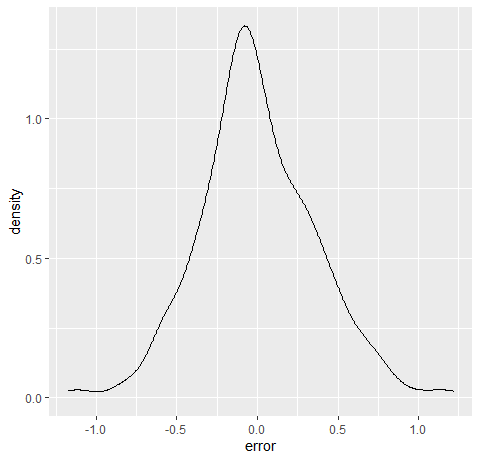
\includegraphics[width=.4\linewidth]{figures/errDist.png} }}
    \qquad
    \subfloat[\centering Q-Q Plot of Errors]{{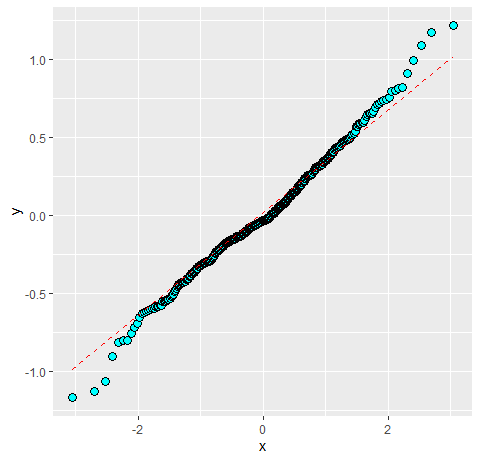
\includegraphics[width=.4\linewidth]{figures/errorqq.png} }}
    \caption{Error distribution with Q-Q plot}
    \label{errDistAndQQ}
\end{figure}

As we can see in this figure, there is a general bell curve, but not quite perfect as we have a bump between -0.5 and -0.75, as well as between 0.125 and 0.5. This 
non-normality is reflected in the Q-Q plot of the error. Measuring accuracy of the results is harder for these value prediction networks is harder than in classification 
problems. This is because we can't construct a prediction matrix. We don't expect the network to predict values down to the exact run, this would require a lot more 
data than is available, and a large amount of experimentation. One metric we can therefore use to see how accurate our model is, is to calculate 
the corrolation between the actual results and the predicted results. Using the inbuilt \textit{cor()} function, we obtain a corrolation value of 
$0.9382$. Given how close this is to 1, which would be perfect corrolation, it is fair to say that this method has done well to predict scores. \\

The issue that one may point out here is that this network has been trained on a full-over dataset, and then been tested on a full-over dataset. But the purpose of this 
investigation has been to look at the scenario in which a full game has been completed. So the method is currently ineffective at doing the task it set out to solve. For this reason,
we must come up with a way to 'fill in' the missing overs. The idea for this is to use Monte-Carlo simmulation. We discussed in \ref{exprr} how depending on the stage of the game,
the runrates can be drawn from one of three normal distributions. So for the overs that are missed, we can simply fill in the gaps by drawing a value from the distribution that the missing over falls 
into. 

\subsection{Interlude: Monte-Carlo Simmulation}
Before simmulating cricket games to test our network on, we first find it necessary to delve into the mathematics of the methods used to for doing the simmulating. This is where
``Monte-Carlo'' simmulating comes in. \\
Let H be some random variable. At this stage, the distribution of H is irrelevant, but we note that $\mu = E(H)$. Formally, we have the following definition.

\begin{definition}
    Let $n \in \mathbb{N}$ and let $\{H_i \ | \ i =1,\ldots,n\}$ be i.i.d copies of H. The \textbf{Monte-Carlo Estimate} of $\mu$, is given as $\hat{\mu}=\frac{1}{n}\sum_{i=1}^n H_i$.  
\end{definition}

Recall the well-known \textit{Strong Law of Large Numbers}.

\begin{theorem}
    \label{slln}
    Let $n \in \mathbb{N}$, and let $H_1$,$H_2$,... be an i.i.d sample from a distribution with expectation $\mu$ and standard deviation $\sigma$, with $\mu, \ \sigma < \infty$.
    Then 
    $$ 
        P\left( \lim_{n \to \infty} \bar{H}_n = \mu \right) = 1
    $$
\end{theorem}

It follows from Theorem \ref{slln} that

\begin{align}
\lim_{n \to \infty} \hat{\mu} &= \lim_{n \to \infty} \frac{1}{n}\sum_{i=1}^nH_i \\
                              &= E(H) \\
                              &= \mu.
\end{align}

\subsection{Match Simulation}
With the theoretical framework for Monte-Carlo simmulation established, we can now look to build an algorithm for simmulating cricket matches. Based on our own work in Chapter 4, 
we begin by defining three random variables, $R_{\text{powerplay}} \sim N(\mu_{\text{powerplay}},\sigma_\text{powerplay})$, $R_{\text{middle}} \sim N(\mu_{\text{middle}},\sigma_{\text{middle}})$
and $R_{\text{final}} \sim N(\mu_{\text{final}},\sigma_{\text{final}})$.

The numerical values for these are given in the following table.

\begin{table}[h]
    \centering
    \begin{tabular}{c | c | c}
        Numerical Values & $\mu$ & $\sigma$ \\
        \hline
        $R_{powerplay}$ & 1.5298 & 0.4486 \\
        $R_{middle}$ & 1.6541 & 0.3355 \\
        $R_{final}$ & 3.1493 & 1.1349 
    \end{tabular}
    \caption{Numerical values of the parameters used for Monte-Carlo simmulation}
\end{table}

The code for doing this simmulation was not hard to write, and after a few small performance enhancements ran almost instantaneously. The code can be seen in figure \ref{mcecode}.

\begin{figure}[h] %MAKE SURE THESE ARE THE RIGHT LINES OF CODE!!
    \label{mcecode}
    \lstinputlisting[language=R, firstline=5,lastline=25]{../code/PyScripts/monteCarlo.py}
    \caption{Implementing a Monte-Carlo Simmulation fo Cricket Matches}
\end{figure}

It is best to think of n as a sort of fine-tuning parameter. If we have n too large, we would simply be simmulating the average cricket game, while have n too low and 
we are open to having an outlier. As for the other parameters, we have \textit{overs} being the number of overs in the game, and \textit{state} determines the over to start 
simmulating from. So if we want to simmulate the whole game, set $state=1$ and $overs=50$. The array \textit{runrates} just holds the data.\\

We then have the function \textit{MCE(n,state)}. The first line of this is a ``Ternary Operator'' to determine a parameter $t$. The job of $t$ is to be an index which obtains 
the correct parameters from the arrays in lines 2 and 3. This is then fed into the next line, uses the \textit{random.normalvariate()} function to populate an empty list with random 
values drawn fro the appropriate distribution of R. This is then averaged and returned by the function. Completing the main part of the Monte-Carlo method.
Finally, a while-loop runs through the overs needed and adds the estimation values to the \textit{runrates} array. \\

To give an idea of how the value of $n$ affects the resulting simmulation, we ran two simulations, using a small value $n=5$, and a larger one using $n=100$. 

\begin{figure}[h]
    \centering
    \subfloat[\centering $n=5$]{{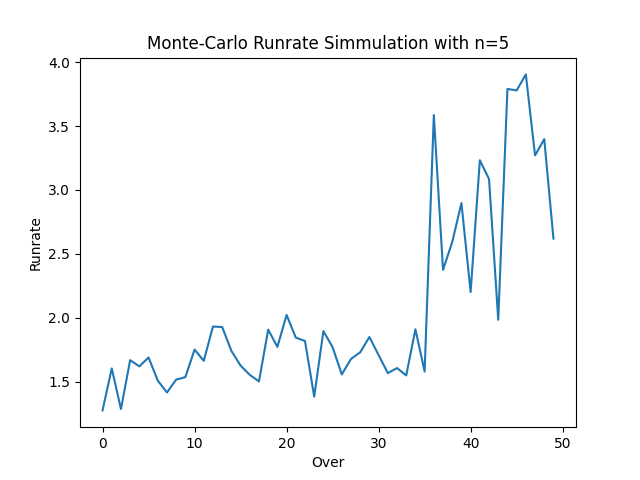
\includegraphics[width=.4\linewidth]{figures/mcen5.png} }}
    \qquad
    \subfloat[\centering $n=100$]{{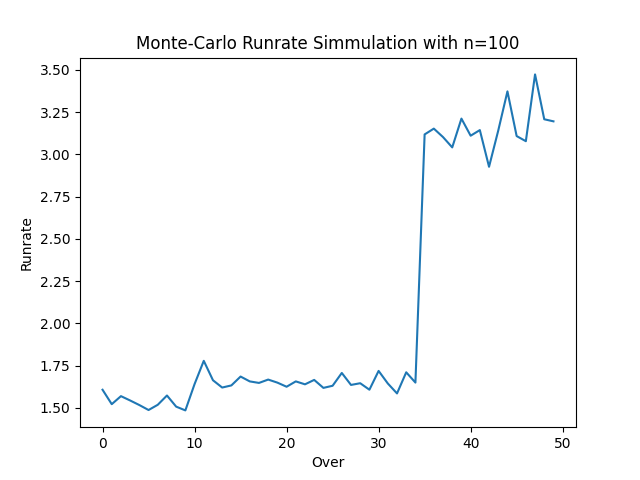
\includegraphics[width=.4\linewidth]{figures/mcen100.png} }}
    \caption{50-Over simmulation of $n=5$ and $n=100$}
    \label{MeanAndSDRR}
\end{figure}

If we compare these figues with (a) in Figure \ref{MeanAndSDRR}, we see that with large $n$, we have fallen victim to the ``Central-Limit Theorem'', and it looks as if the three 
sections of the game are unrelated. In the end, $n=20$ was the chosen value as it provided an appropriate middleground. 

\section{England VS South Africa, 1992 World Cup}
In this section, we take the models that were produced in the prior chapter and apply them to the controversial game at the 1992 Australian Cricket World Cup. In the second semi-final,
played between England and South Africa at the Sydney Cricket Ground. England had not completed their 50 overs by 18:10pm, and so the number of overs was reduced to 45 overs. In South Africa's
innings, rain stopped play 5 balls into over 43. At this point in the game, South Africa were 231/6 with 13 balls left, chasing 253. The game was reduced to 43 overs, and using the \textit{most 
productive overs method}, South Africa were set a target of 252 off 43 overs, leading to the impossible requirement of 21 off 1 ball.\footnote{At the time, the electronic scoreboard at the ground,
and the TV coverage incorrectly displayed 22 to win off 1 ball.}

Note the afforementioned \textit{Most Productive Overs Method} is given by the equation:

\begin{equation}
    \text{Target in X overs} = \text{Runs scored by Team 1 in their highest-scoring X overs} + 1.
\end{equation}

A Duckworth-Lewis calculation was done retrospectively, and would have first set South Africa a target of 273 fron 45 overs, then 257 from the 43 overs.


